\subsection{Motor modelling}
A model of a motor consist of both a mechanical and an electrical section, due to the electrical current, $i_a(t)$, which is converted to a rotational force called torque, $\tau_m$. Therefore a model of the mechanical and the electrical system should be produced. The mechanical model from the motor will provide what the motors contributions to the drivetrain is, see \secref{DriveTrain}, and the electrical model will provide the motors torque.

\subsubsection{Mechanical model}

\begin{figure}[H]
	\centering
	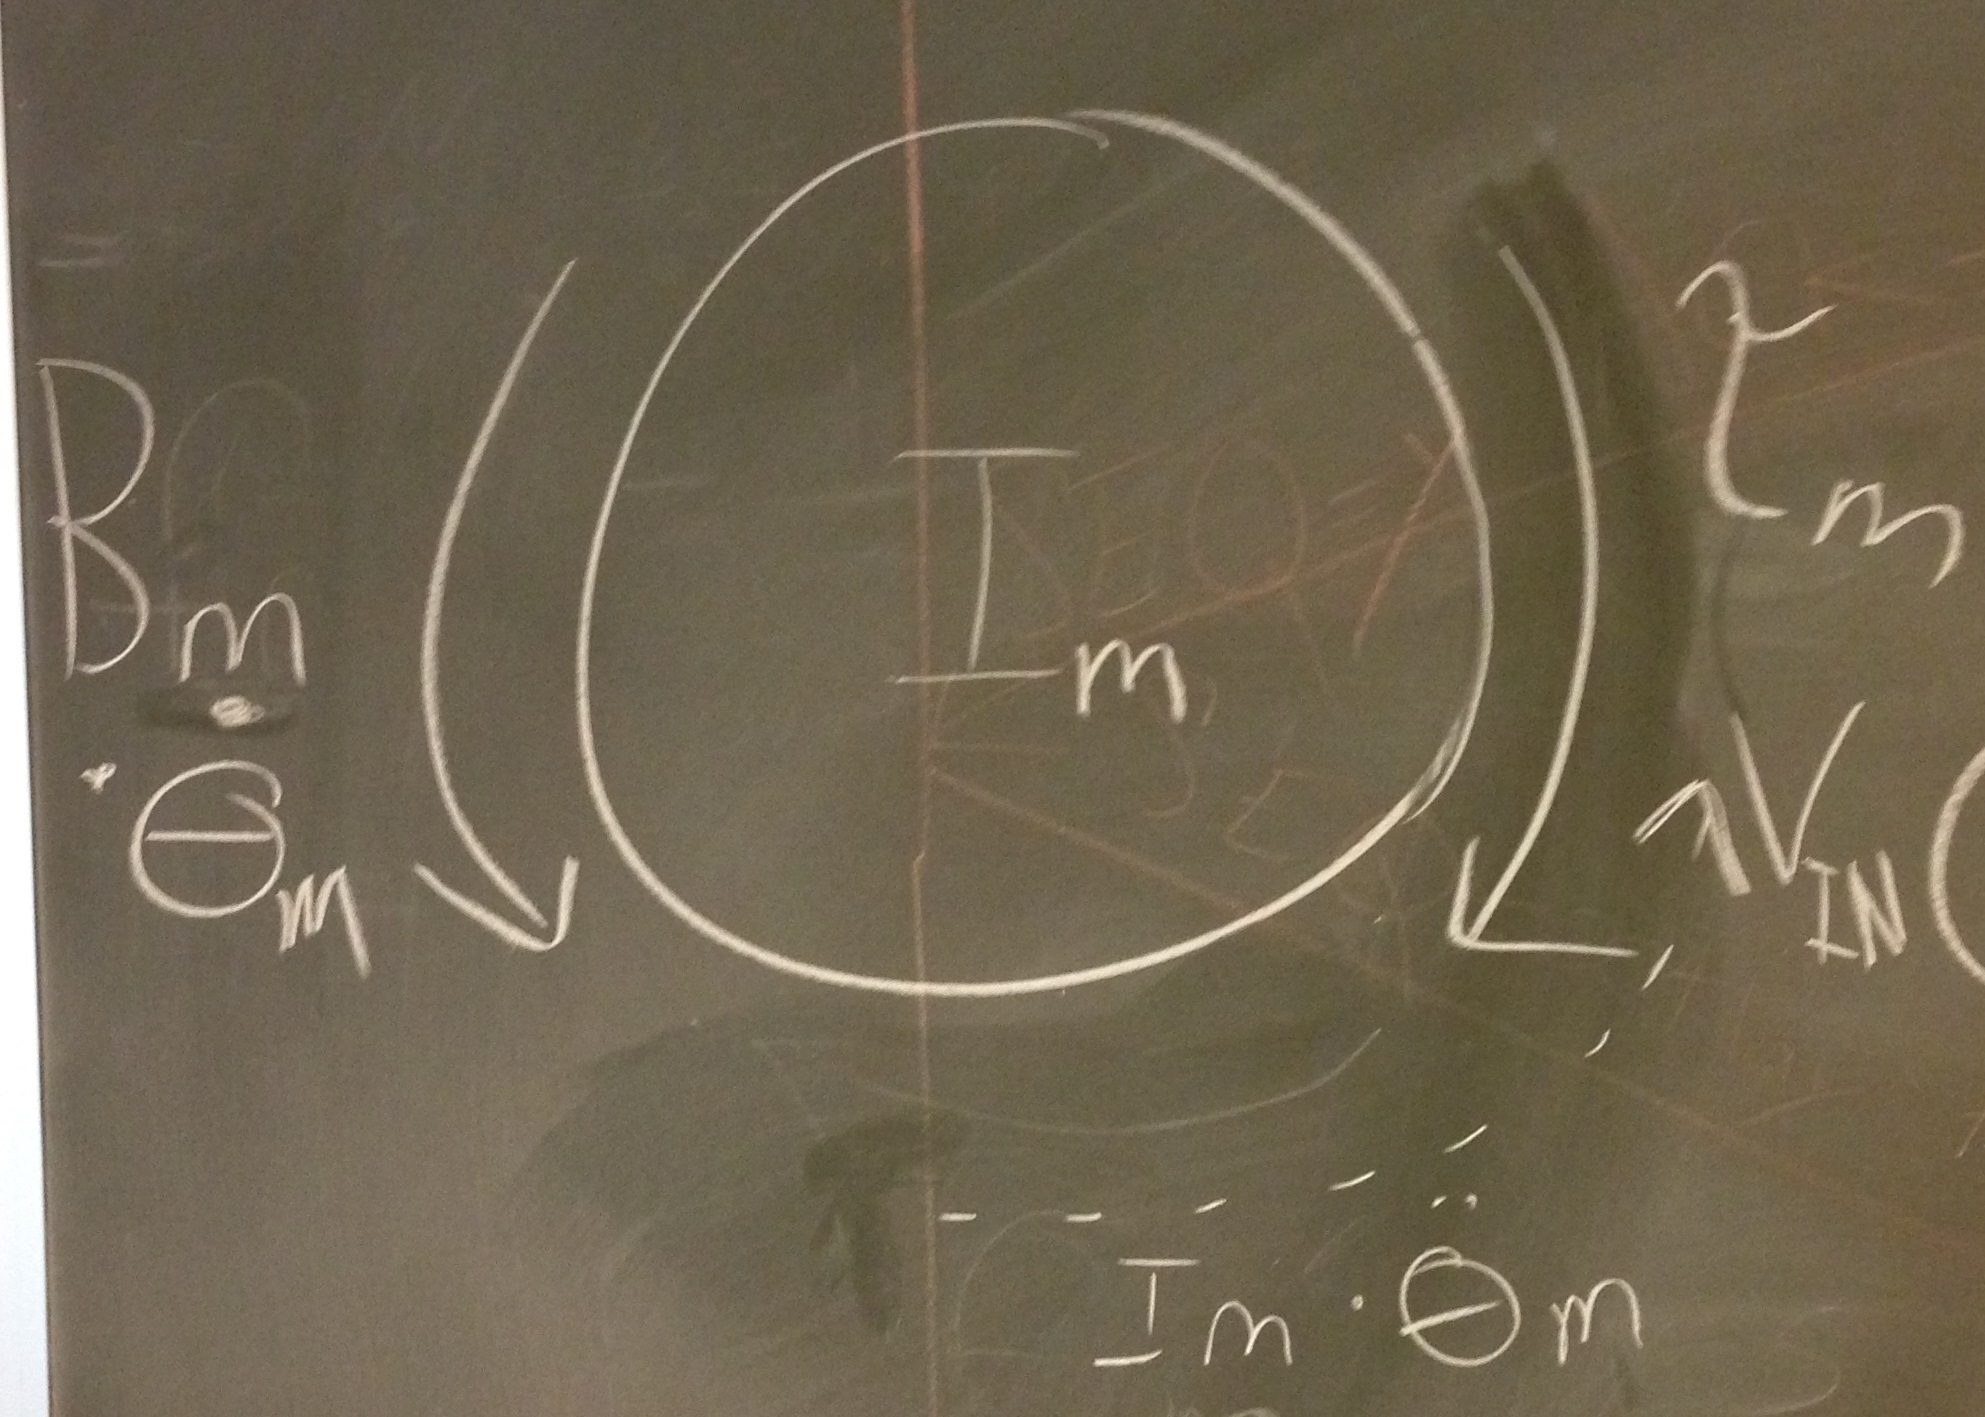
\includegraphics[scale=0.1]{figures/MotorFreeBodyDiagram.jpg}
	\caption{Free body diagram of the motor}
	\label{fig:MotorFreeBody}
\end{figure}

\subsubsection{Electrical model}
The output from the motors electrical model is torque, $\tau_m$. To obtain torque the formula for translating the electrical current, $i_a$, to torque is utilized:

\begin{flalign}\centering
  \tau_m = i_a(t) \cdot K_t %\unit{\volt}
  \label{equ:motortorque}
\end{flalign}
\hspace{6mm} Where:\\
\begin{tabular}{p{1cm}ll}
& $\tau_m$ & the rotational force torque [$N \cdot m$] \\
& $i_a(t)$ & the electrical closed loop current [$A$]\\
& $K_t$ & the torque constant [$\frac{N \cdot m}{A}$] \\
\end{tabular}

An expression for the current, $i_a$, is required to derive a model for the electrical system. In \figref{fig:MotorElectric} an electrical diagram of the motor is display.

\begin{figure}[H]
	\centering
	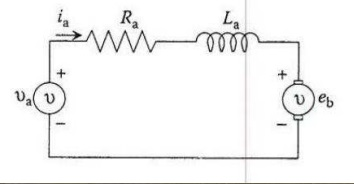
\includegraphics[scale=0.8]{figures/MotorElektrikDiagram.jpg}
	\caption{Electric diagram of the motor}
	\label{fig:MotorElectric}
\end{figure}

By using Kirchoffs voltage law on the closed loop, seen in \figref{fig:MotorElectric}, an expression for $i_a$ can be derived:

\begin{flalign}\centering
V_a(t) = R_a \cdot i_a(t) + L_a \cdot \frac{di_a}{dt} + e_b 
\label{MotorClosedLoop}
\end{flalign}
\hspace{6mm} Where:\\
\begin{tabular}{p{1cm}ll}
& $V_a(t)$ & the supply voltage [$V$] \\
& $R_a$ & the eternal resistance in the motor [$\Omega$]\\
& $L_a$ & the inductance in the motor [$H$] \\
& $e_b$ & the electromotive force, also called EMF [$\V$] \\
\end{tabular}

The electromotive force, $e_b$, is equivalent to:

\begin{flalign}\centering
e_b = K_e \cdot \dot{\theta}_m 
\end{flalign}
\hspace{6mm} Where:\\
\begin{tabular}{p{1cm}ll}
& $K_e$ & the electromotive constant [$Wb$] \\
& $\dot{\theta}_m$ & the angular velocity in the motor [$\frac{rad}{s}$] \\
\end{tabular}

the equivalent for the electromotive force is substituted into \eqref{MotorClosedLoop}.

\begin{flalign}\centering
V_a(t) = R_a \cdot i_a(t) + L_a \cdot \frac{di_a}{dt} + K_e \cdot \dot{\theta}_m(t)
\end{flalign}

The Laplace transform is applied to the derived equation:

\begin{flalign}\centering
V_a(s) = R_a \cdot i_a(s) + L_a \cdot s \cdot i_a{s} + K_e \cdot \dot{\theta}_m(s) 
\end{flalign}

